\section{Interval Vertex Coloring (IVC)}
\subsection{Vertex Color Problem}
\begin{frame}{VCP}
  \begin{columns}
    \column{.6\textwidth}
      \begin{itemize}
        \item<1-> Given G(V,E)
        \item<2-> Find a vertex coloring s.t. colors on adjacent vertices differ
      \end{itemize}
      \begin{block}{Formal Definition of VCP given G(V,E)}<3->
        $\text{find} \, f(v):$
        $\forall v\in V:\forall w \, in \, \Gamma(v): f(v) \neq f(w).$
      \end{block}
      
    \column{.4\textwidth}
    \centering
    
    
    \null
    \centering
      G(V,E)
      \null
      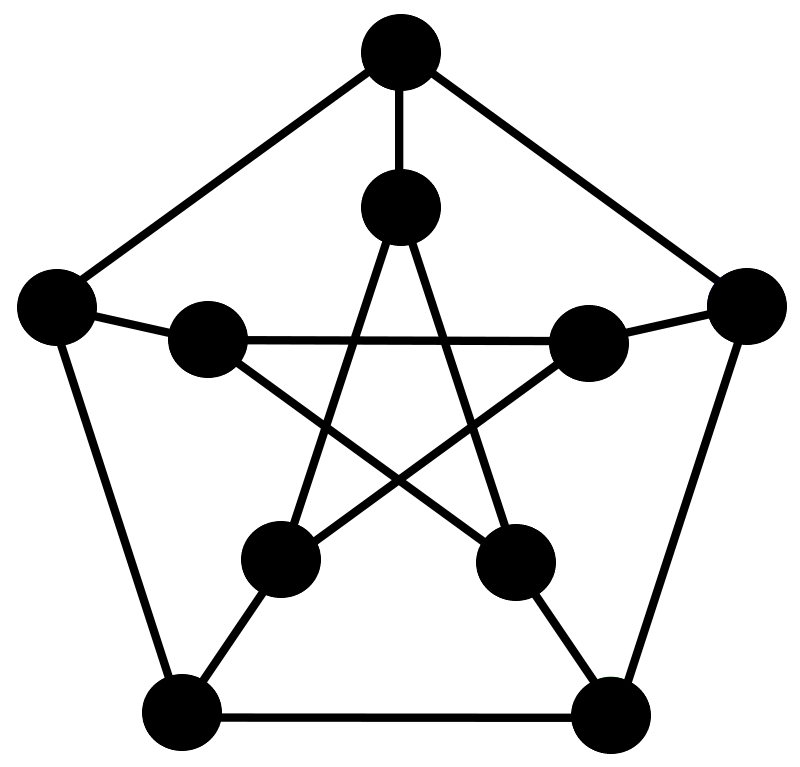
\includegraphics[width=0.8\textwidth]{figures/graph_coloring1.png}<1->
      \null
      \null
      \onslide<4->{Colored G(V,E)}
      \null
      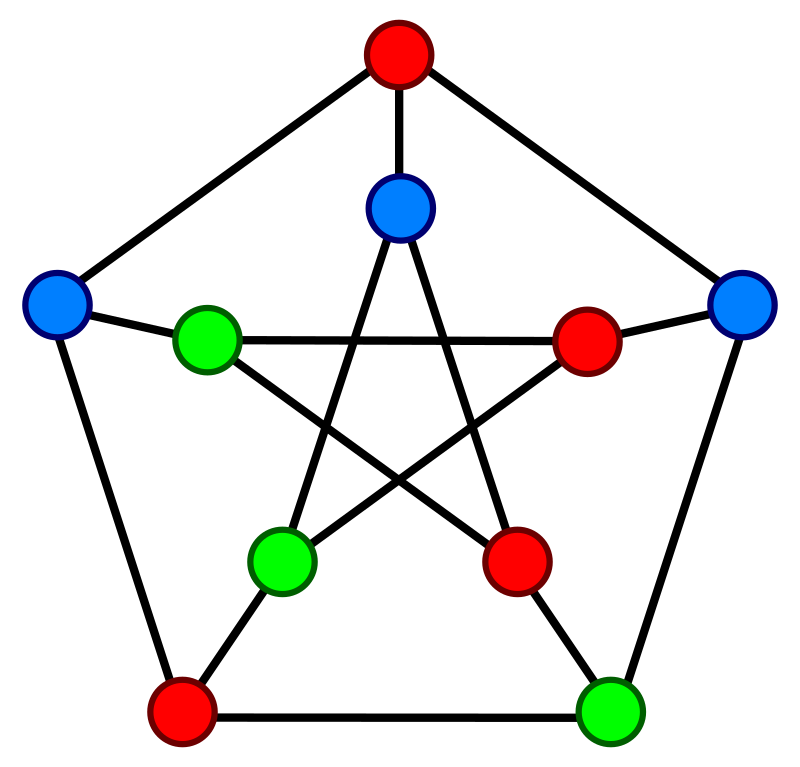
\includegraphics[width=0.8\textwidth]{figures/graph_coloring.png}<4->
  \end{columns}
\end{frame}

\subsection{Interval Vertex Coloring Problem}
\begin{frame}{IVC}
  \begin{columns}
    \column{.4\textwidth}
        \centering
        G(V,E) \\
        \null
        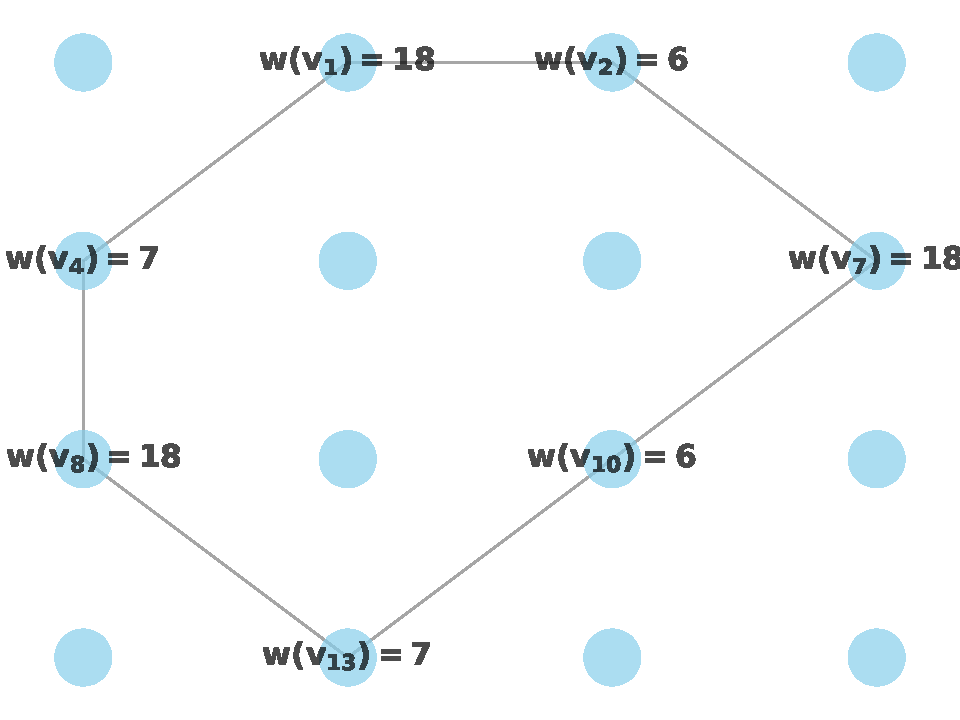
\includegraphics[width=1\textwidth]{figures/ICV0.pdf}<1-> \\

    \column{.6\textwidth}
    \begin{itemize}
      \item<1-> Let G(V,E) be an undirected graph and $w : V \mapsto \mathbb{Z^+}$ the weights.
      \null
      \vfill
      \null
      \item<2-> A interval coloring of the vertices of G is a function $\text{start} : V \mapsto \mathbb{Z^+}$
      \null
      \vfill
      \null
      \item<3-> Vertex v is colored with open interval:
      $[\text{start}(v), \text{start}(v)+w(v))$
      \null
      \vfill
      \null
      \item<4-> Neighboring Vertices must have disjoint color intervals: 
      $\forall (a, b) \in E:$ \\
      $ [\text{start}(a), \text{start}(a) + w(a)) \cap [\text{start}(b), \text{start}(b) + w(b)) = \emptyset.$
      
    \end{itemize}
  \end{columns}
\end{frame}

\begin{frame}{Formal IVC Problem Definition}
  \begin{columns}
    \column{.4\textwidth}
        \centering
        \onslide<3->{Interval Colored G(V,E) with maxcolor = 30} \\
        \null
        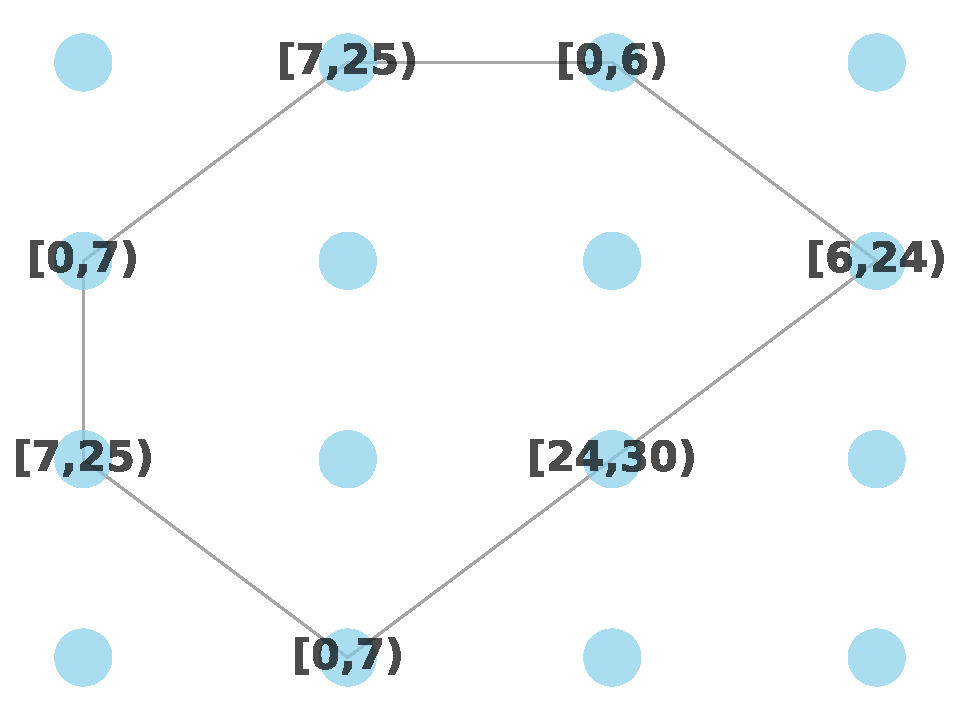
\includegraphics[width=1\textwidth]{figures/ICV1.pdf}<3->
    \column{.6\textwidth}
    \begin{itemize}
      \item<1-> A interval coloring of the vertices of G is a function $\text{start} : V \mapsto \mathbb{Z^+}$
      \null
      \vfill
      \null
      \item<2-> A particular coloring "start" of the vertices of G is said to use:
      \[ \text{maxcolor}= \max_{v \in V} start(v) + w(v) \hspace{0.25cm}  \text{colors.}\]
    \end{itemize}
      \begin{block}{Optimization Problem Instance:}<4->
        Find a coloring $\text{start}:V \mapsto \mathbb{Z}^+$ that minimizes maxcolor. \\
      \end{block}
      \null
      \vfill
      \null
    \begin{itemize}
      \item<4-> A maxcolor that is indeed minimal, is denoted with maxcolor* .
    \end{itemize}

  \end{columns}
\end{frame}
  




  % \subsection[Paragraphs]{Simple Paragraphs}
  % \begin{frame}[fragile]
  %   \frametitle{Title first category}
  %   \framesubtitle{Title second category}
  %   % no deeper title hierarchy provided 
  %   You can cite~\cite{Tan11}. Urls look like this: \url{http://www.google.com/}.
  % \end{frame}